\documentclass{kththesis}


%Taken from ID1354
\usepackage[utf8]{inputenc}
\usepackage[english]{babel}
\usepackage{graphicx}
\usepackage{lastpage}
\usepackage{pgf}
\usepackage{wrapfig}
\usepackage{fancyvrb}
\usepackage{fancyhdr}
\pagestyle{fancy}
\usepackage{dingbat}

\usepackage[autostyle]{csquotes}
\usepackage[
    backend=biber,
    style=ieee,
    sortlocale=de_DE,
    natbib=true,
    url=true,
    doi=true,
    eprint=false
]{biblatex}
\addbibresource{references.bib}

\usepackage[]{hyperref}
\hypersetup{
    colorlinks=true,
}

% List of abbreviations
\usepackage{glossaries}
\makeglossaries

\title{Extending Timing Analysis for Non-Preemptive Task Sets on Multicore Under the AER Model}
\alttitle{Detta är den svenska översättningen av titeln}
\author{Jacob Kimblad}
\email{jacobki@kth.se}
\supervisor{Matthias Becker}
\examiner{Zhonghai Lu}
\programme{Master's Programme in Embedded Systems}
\school{School of Electrical Engineering and Computer Science}
\date{\today}


\begin{document}

%Term definitions
\newacronym{os}{OS}{Operating System}
\newacronym{cpu}{CPU}{Central Processing Unit}
\newacronym{lcu}{LCU}{Central Processing Unit}
\newacronym{aer}{AER}{Acquisition Execution Restitution}
\newacronym{cots}{COTS}{Commerical off the Shelf}
\newacronym{edf}{EDF}{Earliest Deadline First}
\newacronym{rms}{RMS}{Rate-Monotonic Scheduling}
\newacronym{lcm}{LCM}{Least Common Multiple}
\newacronym{bcet}{BCET}{Best-Case Execution Time}
\newacronym{wcet}{WCET}{Worst-Case Execution Time}
\newacronym{prem}{PREM}{PRedictable Execution Model}
\newacronym{gprem}{gPREM}{global PREM}
\newacronym{ilp}{ILP}{Integer Linear Programming}
\newacronym{dms}{DMS}{Deadline Monotonic Scheduling}
\newacronym{autosar}{AUTOSAR}{AUTomotive Open System ARchitecture}
\newacronym{ecu}{ECU}{Electronic Control Unit}

% Frontmatter includes the title page, abstracts and table-of-contents
\frontmatter

\titlepage

\begin{abstract} 

    English abstract goes here.

\end{abstract}


\begin{otherlanguage}{Swedish} 
    
    \begin{abstract}

    \end{abstract} 

\end{otherlanguage}

% List of Acronyms
\printglossary[title={Acronyms}]

% Table of contents
\tableofcontents

% Mainmatter is where the actual contents of the thesis goes
\mainmatter


\chapter{Introduction} 
Embedded systems in the automotive sector are required to go through a lot of analysis and testing
before being deemed safe for use in traffic. With the rise of autonomous vehicles these systems are
becoming more complex as an effect of more computing needed being done.  This has also put
requirements on the hardware to become faster and faster, thus the industry is turning to the use of
multi-core and many-core platforms. These type of platforms present more unpredictability than
single-core platforms which requires new methods of analysis and deterministic execution of these
systems. 


\section{Background} 

Timing analysis is an important part of real-time systems. However, multi-core platforms often
implement complicated memory hierarchies that make timing analysis a lot harder. One way to tackle
this is to schedule the access to shared memory in cooperation with computational tasks. This can
improve analysis and is employed by industrial domains already where the execution of tasks can be
divided up into three distinct parts, read-execute-write.


\section{Problem}

An analysis method for resource contention in multi-core real-time systems have been proposed in
paper [1]. This analysis method is however not customised for the read-execute-write execution model
that is adapted both within the avionics domain and automotive domain.


\section{Purpose}

The purpose is to expand existing analysis methods by adding to the source code and/or produce a
model of the read-execute-write task model that is available as input for these formal analysis
methods.


\section{Goal}



\subsection{Benefits, Ethics and Sustainability}

\section{Methodology / Methods}

\section{Delimitations}

\section{Outline}


%We use the \emph{biblatex} package to handle our references.  We therefore use the command
%\texttt{parencite} to get a reference in parenthesis, like this \parencite{heisenberg2015}.  It is
%also possible to include the author as part of the sentence using \texttt{textcite}, like talking
%about the work of \textcite{einstein2016}.

\chapter{<Theoretic Background> Use a self-explaining title}



\section{The Task Model} \label{sec:the_task_model}

%TODO Maybe add a picture that shows all the characteristics of a job/task
A periodic task, denoted as $\tau_i$, is a unit of work that is executed periodically on a processor
alongside other tasks over and over again. In embedded systems a task is usually completed in some
amount of time known as its \textbf{computation time}, denoted as $C_i$. Once a task has finished
executing it will usually wait for some amount of time before it is ready to execute again, this is
known as the tasks \textbf{period}, denoted by $T_i$. The earliest time where a task is ready to
start execution within a new period is called the \textbf{arrival time} of the task and is denoted $
a_i $. Note that the arrival time is equal to the beginning of the current period of the task.

The \acrshort{lcm} of the periods for all the tasks in a task set is known as the task set's
\textbf{hyper-period} and is an important concept in scheduling tasks which is further discussed
in section \ref{sec:scheduling}. The hyper-period is defined as $H = \acrshort{lcm}(P_i)$ for $i =
1, 2, ..., n$. Each task is also required to finish execution before a set amount of time starting
from each new period belonging to the specific task, this is known as the task's \textbf{relative
deadline} denoted as $D_i$. For an \acrshort{os} to decide in what order the tasks should execute
when more than one is available at the same time they are each assigned a \textbf{priority}, denoted
by $P_i$, by a scheduler which is further discussed in section \ref{sec:scheduling}. A task can thus
be introduced by defining its characteristics as $\tau_i = (C_i, T_i, D_i)$. It is then also possible to
define a task set as $ \Gamma = \{\tau_1, \tau_2, \tau_3, ..., \tau_n\} $.

Following the above definitions state can be can ascribed to tasks depending on their status in the
system at a specific time instance. A task is in the \textit{ready} state when it still needs time
to complete its execution before its deadline but is not yet allowed access to the processor. Once a
task is moved out of the ready state and is executing on the \acrshort{cpu} it is said that the task
is \textit{running}. The task can also be moved back to the ready state from running state before
execution is finished by being \textbf{preempted} by the scheduler. If a task requires access to
some shared resource that is not currently available, thus halting execution, the task is said to be
\textit{waiting}. Once the shared resource is available again the task is moved back into the ready
state. The three different states and their transitioning are depicted in figure
\ref{fig:ready_running_blocked_model}.

\begin{figure}

    \centering

    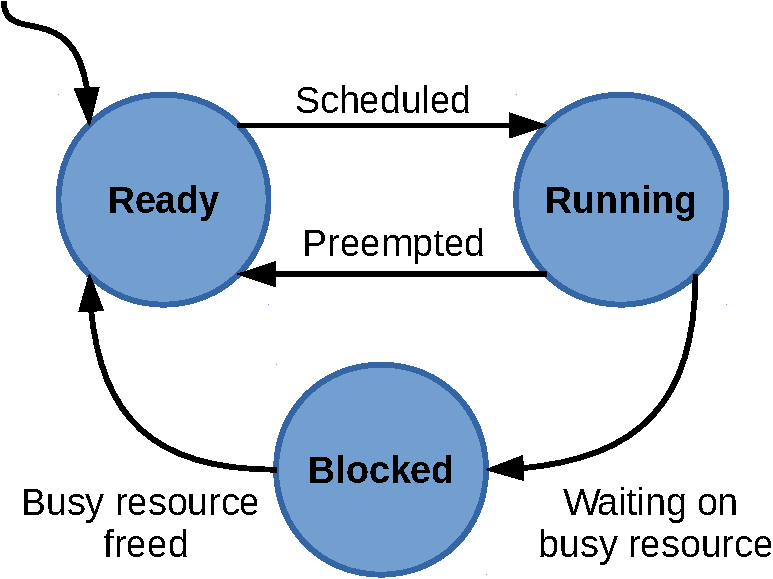
\includegraphics[width=0.7\linewidth]{images/ready-running-blocked-model.pdf}

    \caption{The three states a task may be in.}

    \label{fig:ready_running_blocked_model}

\end{figure}

The task model presented thus far has made some assumptions that are not realistic, such as the
release time and computation time being exactly the same each period. In order for the model to
better represent reality to increase the validity of schedulability analysis methods some additional
concepts are introduced. Computation time of a task varies because of unpredictable behaviour in the
processor such as caches. Therefor the notions of \acrfull{bcet} and \acrfull{wcet} is introduced to
represent the interval between the fastest and the slowest computation time of a specific task.  To
denote this $ C_i^{min} $ and $ C_i^{max} $ is used. In addition to uncertainties in the computation
time there are also uncertainties in the arrival time of tasks. The notion of earliest arrival time,
denoted $ a_i^{min} $, is the  absolute earliest time at which a task may be able to start executing
within the period and likewise the latest arrival time, denoted $ a_i~{max} $ is the time when the
task is guaranteed to be able to start execution. In addition, the intervals for computation times
and release jitter can be represented as a probability distribution, but this will not be covered in
this thesis.


% TODO: Introduce the notion of offline and online schedulers, start time of tasks (when they start
% execution)
\section{Scheduling} \label{sec:scheduling}

Although computers give away the illusion of being able to deal with many things simultaneously this
is actually not the case. Computers are limited to how much parallel computing they are able to do
by the hardware, specifically the amount of cores within the \acrshort{cpu}. A computer with, for
example, a single core \acrshort{cpu} is only able to execute one task at a time. For a computer
with a single core to deal with more than a single task at the same time requires switching ongoing
tasks in and out of the core during runtime. For the \acrshort{os} to switch tasks quickly in and
out of the core it needs to schedule the tasks according to some order. This is where the priority
of tasks come in handy, by scheduling tasks and switching them in and out of the processor very
quickly depending on their priority the \acrshort{os} is able to perform more than one task seemingly in
parallel than what is actually allowed for by hardware. The rest of this section up until section
\ref{subsec:multiprocessor_scheduling} is only concerned with the scheduling of single core
processors.

% TODO Maybe add other measurements of how good schedulers are, least-slack time etc.
The order in which tasks are executed is determined by the scheduler which in of itself is a special
type of task executed by the \acrshort{os}. The scheduler is invoked by specific events happening in
the system. It could for example be that a task is finished executing or that it has begun waiting
on some resource that is not yet available. As not all scheduling algorithms were created equal they
vary in how good of a task they do when scheduling the same task sets. Because of this some
measurements must be introduced in order to have a fair comparison of how well they work. The
processor utilization factor, denoted as $ U $, is such a measurement introduced to show to what
percentage a specific task set would keep the processor busy. The utilization can be calculated as
$ U = \sum_{i=1}^n \frac{C_i}{T_i} $.

For embedded systems there exists a set of well known scheduling algorithms such as \acrshort{edf}
and \acrshort{rms}. Imagining a single-core \acrshort{cpu} the algorithm \acrshort{rms} works by
setting the priority of each task equals to its period. This means that the task with the lowest
period is given the highest priority and always scheduled first once it is in the ready state. Since
periods of tasks never changes during execution, the priorities of the individual tasks will never
change either, thus \acrshort{rms} is said to be a \textbf{static-priority scheduler}. If a
scheduler instead changes the priorities of the task during execution it is a
\textbf{dynamic-priority scheduler}. 

Instead of setting priorities according to the periods, \acrshort{edf} works by setting the
priorities according to how close a task is to its deadline. This means that the task closest to
exceeding its deadline will always be executing first on the processor. If some task $ \tau_a $ is
executing with a deadline further away in time than another task $ \tau_b $, that was just released,
then $ \tau_a $ will get preempted and the newly released $ \tau_b $ will be allowed to execute
instead. This behaviour makes \acrshort{edf} a \textbf{preemptive scheduling algorithm}, the
opposite of which is a \textbf{non-preemptive scheduling algorithm} which lets each task finish
before scheduling the next highest priority task.

An example of how \acrshort{rms} would schedule a task set can be seen in figure
\ref{fig:rate_monotonic_scheduling}. A special point of interest is at time 4 when $T_3$ is
executing since earlier as $T_1$ is released. Due to $T_1$ having a lower period than $T_3$ it also
has a higher priority. The scheduler preempts $T_3$ and lets $T_1$ execute instead. $T_3$ is later
allowed to resume execution of $j_3$ at time 5.

\begin{figure}

    \centering

    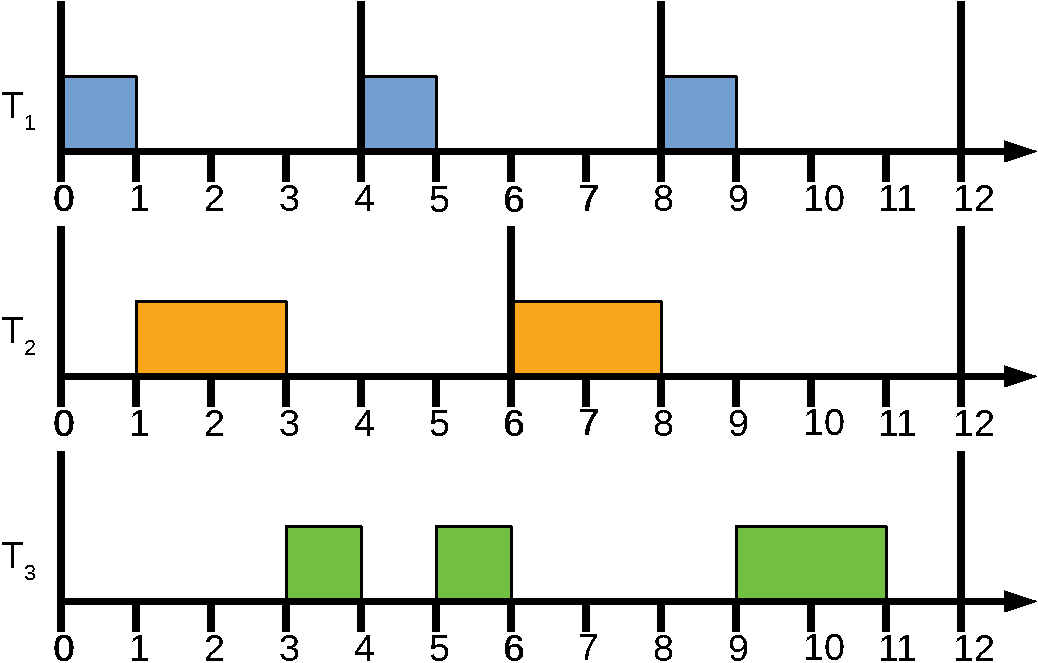
\includegraphics[width=0.8\linewidth]{images/rate-monotonic-scheduling.pdf}

    \caption{Example of rate monotonic scheduling for three tasks where $T_1=(1, 4, 4)$, $T_2=(2, 6,
    6)$, $T_3=(4, 12, 12)$.}

    \label{fig:rate_monotonic_scheduling}

\end{figure}

When dealing with non-preemptive single-core systems where the tasks periods equal the tasks
deadlines \acrshort{rms} guarantees finding a feasible schedule if such a schedule exists, making it
an \textbf{optimal} scheduling algorithm. For preemptive single-core systems, \acrshort{edf} has
been proven to always find a feasible schedule if one exists, making it optimal in those
circumstances. If an algorithm however is unable to find a feasible schedule, even when such a
schedule exists, it is considered a \textbf{heuristic}.

\subsection{Multiprocessor scheduling} \label{subsec:multiprocessor_scheduling}

When considering multi-core processors life for schedulers become a little harder. On a single-core
processor the scheduler only needs to consider temporal allocation of the task, as in
\underline{when} they should run. Scheduling tasks on a multi-core system also requires the
scheduler to consider spatial allocation of the tasks, as in \underline{where} they should run
(on what core). Schedulers deal with these allocations in two different ways, either through what is
known as \textbf{global scheduling} or through \textbf{partitioned scheduling}. 

%TODO: Mention some examples of multi-core scheduling algorithms (gEDF, RMS, etc)
%TODO: maybe have pros and cons for partitioned and global scheduling
%TODO: Maybe have a picture to help explain the differences between partitioned and global
%scheduling. This contains a good example:
%http://retis.sssup.it/~giorgio/slides/cbsd/mc3-global-2p.pdf
Partitioned scheduling entails that each task is assigned to a dedicated core where it always will
be running. Due to this any single-core scheduling algorithm can be used individually on each core
during runtime. It is then possible to also use the existing scheduling analysis methods for the
respective scheduling algorithm.  This sounds easy enough, but in reality assigning tasks to cores
is a version of the bin packing problem which is known to be a NP-hard problem meaning that there
exists no algorithm to solve it in less than polynomial time. However, good heuristics
\parencite{johnson_fast_1974}\parencite{coffman_application_1978} exists that find good solutions
fast and since tasks can be allocated to cores offline more computing power can be used to find
close to optimal solutions in reasonable time.

Global scheduling means that the scheduler takes into account both spatial and temporal allocation
when scheduling each task. Algorithms from sing-core scheduling can be applied to global scheduling
such as \acrshort{rms} and \acrshort{edf}, but they will have different behaviour. Global scheduling
decreases the determinism of the system and creates more combinations of possible schedules for each
task set.

\section{Schedulability analysis}

%TODO mention brute-forcing analysis by simulating one hyper period of the schedule. And this seems
%easy in theory, but in practice there can be hundreds of tasks and super long hyper period.
When developing new scheduling methods it is important to put the schedules that they produce under
analysis as to show whether they are feasible or not. It is especially important when the schedules
are used in hard real-time systems like those found in the avionics and the automotive sector where
missed deadlines could mean fatal outcome. For example, \acrshort{rms} can be analysed
mathematically and has been proven to be able to schedule any task set that fulfills the constraint
$ U \le n(2^{\frac{1}{n}}-1) $ where $ n $ is the amount of tasks \parencite{liu_scheduling_1973}.
This is only a \textbf{sufficient} condition, meaning that \acrshort{rms} might be able to schedule
task sets that do not fulfill the condition, but it is not guaranteed to. A condition that must be
fulfilled for the task set to have a feasible schedule, but does not guarantee such a schedule
exists, is known as a \textbf{necessary} condition. If a condition is both necessary and sufficient
it is said to be \textbf{exact}. An example of an exact condition for \acrshort{edf} is $ U(\Gamma)
\leq 1 $ which states that the utilization of the task set must be one or less. Finding good
conditions is not always trivial as shown by \parencite{bini_hyperbolic_2001} which presents a less
pessimistic sufficient condition of the same complexity $ O(n) $ for \acrshort{rms} almost 30 years
after the earlier presented condition was introduced. 

%TODO: Mention that increase of tasks leads to harder schedulability
%TODO: Mention that the illustration is mostly to get and idea of the problem trying to be solved,
%and that it represents single-core and a multi-core representation would look slightly different
%(due to a single task not being able to utilize all cores), but the idea is the same.
The gap between sufficient conditions and necessary conditions where the tasks sets are undetermined
if they are able to be scheduled is illustrated in figure
\ref{fig:sufficient_necessary_schedulability}. A lot of research is being aimed towards finding less
pessimistic necessary and sufficient conditions for multi-core scheduling algorithms to close the
gap between them which is still not a solved problem. In addition, each unique scheduling algorithm
may require its own set of unique conditions for analysis. All conditions are also not as simple as
the one presented for \acrshort{rms} especially when considering multi-core. The conditions have
varying complexity and they often need to make the trade-off between complexity and how pessimistic
they are. The paper \parencite{bertogna_tests_2011} shows examples of conditions that are of $
O(n^3) $ complexity which can be alright when analysing small task sets, but is too complex as the
task sets grow or if it has to be calculated online with limited computation power.

\begin{figure}

    \centering

    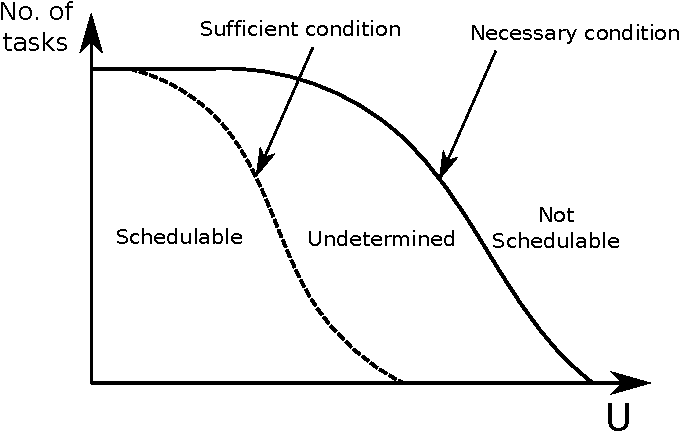
\includegraphics[width=0.8\linewidth]{images/sufficient_necessary_schedulability.pdf}

    \caption{Research aims to shrink the gap left between sufficient and necessary conditions.
    Illustration inspired by \parencite{sebestyen_simulation-based_2012}.}

    \label{fig:sufficient_necessary_schedulability}

\end{figure}

% TODO: Is this section really necessary? Perhaps preface with it by explaining there are different
% ways of analysis. Other than mathematically, we can also simulate the schedule and look for missed
% deadlines. Don't use the word simulation, we are only doing analysis, otherwise people will be MAD
An example of a precise schedulability test for \acrshort{rms} on single-core systems is to find the
so called \textbf{critical instant} of a task. This is when all higher priority tasks are released
at the same time as the task. This pushes the task completion time as far away from its release time
as it ever will be in the given task set. If the task doesn't miss its deadline after the critical
instant it is guaranteed to never miss its deadline for any other instance in the schedule. As an
effect of this, each task can be examined during its critical instant, and if all tasks meet their
deadlines the task set is guaranteed to be schedulable. This facilitates analysis considerably as
only a small part of the schedule needs to be analysed.

Having the arrival and computation time defined as intervals creates the possibility of different
schedules for the same task set using the same scheduler. This makes analysis more difficult as
simulation requires testing several of the combinations of release and computation times. It is
intuitive to think that it is sufficient to analyse the worst-case times of all tasks to find if the
schedule is feasible. This is however not true for non-preemptive systems as two jobs released
within the same interval can lead to either being scheduled until its completion before the other.
For some task sets with this property an earlier release of a certain job can lead to a missed
deadline later in the schedule in multi-core systems. This also means that examining the critical
instant of a task is no longer sufficient in determining if a task set is schedulable or not.
% TODO Example of how earlier release of a task on multicore systems can make the schedule miss a
% deadline while a later release of the same task may have been able to complete the deadline.


\section{The AER Execution Model}

The \acrfull{aer} execution model was first proposed in \parencite{durrieu_predictable_2014} to
improve performance and predictability while using \acrshort{cots} multi-core processors with shared
and private memory in the avionics industry. It builds on top of the \acrfull{prem} first presented
in \parencite{pellizzoni_predictable_2011} which introduces the idea of dividing tasks into a memory
access phase and an execute phase. Since the bottleneck for utilization in multi-core systems can
become the contention in access to shared memory when introducing an increasing number of cores
\acrshort{aer} focuses on making shared memory access more deterministic and easier to analyse. This
is done by dividing up each task into three distinct parts. The \textbf{acquisition} (A) part reads all
the data necessary for execution of the task such as code and shared variables into the private
memory of the core dedicated for execution. The \textbf{execution} (E) phase then executes the code,
without making any further read or write instructions to the shared memory, operating on local
copies of the shared variables. The \textbf{restitution} (R) phase then writes back all of the acquired
results of the task to the shared memory. Since the A-phase only is allowed to execute before
execution of the task actually starts a pre-requisite of the model is that each core has a separate
private memory, such as a cache or a scratchpad. Since these types of memory often are constrained
in size it puts a limit to how many instructions a task can consist of in addition with the amount
of share variables that is used as they all must fit in the private memory of the core.

The idea of this model is to enable scheduling of the read and write accesses to the shared memory
instead of scheduling the tasks onto cores. Since contention of the shared memory is what limits the
utilization of the cores it is more important to combat this instead of trying to find the optimal
assignment of tasks onto cores since it wont increase utilization anyways. \acrshort{aer} can be
said to employ a \textit{memory-centric} approach to scheduling instead of a \textit{core-centric}
approach that schedulers usually employ. Since no reads and writes to shared memory is allowed
outside of the allocated phases a non-preemptive scheduling algorithm is a pre-requisite for the
\acrfull{aer} model. This model also have the advantage of easier analysis by being more
deterministic. When several cores compete for resources and create congestion which leads to timing
deviations the system model becomes more complex thus harder to analyse. Timing that was calculated
offline, for example the \acrshort{wcet}, may not match reality or require very pessimistic
approximations that exaggerate the timings, both of which decreases the certainty or predictability
of the design and analysis.

The scheduling algorithm proposed in \parencite{durrieu_predictable_2014} to schedule the memory
accesses is a partitioned non-preemptive offline algorithm. The paper \parencite{maia_closer_2016}
further evaluates the \acrshort{aer} model by testing different scheduling algorithms. Instead of
using offline partial scheduling it proposes five different heuristic algorithms under online global
scheduling. These algorithms assign a higher task priority according to period (\acrshort{rms}),
shortest acquisition phase, longest acquisition phase, shortest restitution time and longest
restitution time. It is shown through analysis that the \acrshort{rms} scheduler is far best in
terms of schedulable task sets as their utilization increases. The paper
\parencite{becker_contention-free_2016} explores further ways of scheduling under an \acrshort{aer}
model by proposing a global scheduling algorithm that is shown to only behave 0.5\% worse than an
optimal \acrshort{ilp} algorithm in a fraction of the time.

% AER is an improvement over other models such as proposed by pikeOS which enables all other cores
% to be paused while running critical tasks on a single core.


\section{Related Work}

The most important paper to discuss is \parencite{nasri_response-time_2018} which provides a
state-of-the-art schedulability analysis method for non-preemptive static-priority tasks sets under global
scheduling. The analysis is sufficient for multi-core systems and a corresponding precise method for
uni-core systems by the same authors is presented in \parencite{nasri_exact_2017}. The paper is
explained in detail in section \ref{subsec:artafnpjsug}. Since the thesis builds on top of the
concept of the \acrshort{aer} model it is necessary to be familiar with the paper
\parencite{durrieu_predictable_2014} which was the first to present this model and presents an
offline non-preemptive partitioned scheduling algorithm to schedule the memory accesses. The idea to divide
up tasks into distinct execution phases is not a novel one as \acrshort{aer} builds on top of the
\acrshort{prem} which divides up tasks into a read and execute phase for single-core system and was
first presented in \parencite{pellizzoni_predictable_2011}. The \acrshort{aer} model is
further explored in \parencite{maia_closer_2016} which presents five new global non-preemptive
online scheduling algorithms where the most successful assigns priorities to tasks based on their
period in the same way \acrshort{rms} works. It is also shown to be able to schedule tasks sets that
would otherwise not be schedulable under global \acrshort{edf} due to congestion.

%TODO: Mention that this does no take into the account the deadline of the R-phase.
%TODO: Maybe keep all related work covering scheduling analysis in a new subsection
Some work on analysing have been done on analysing the schedulability of algorithms developed around
\acrshort{prem} such as \parencite{alhammad_schedulability_2014} which builds on the idea of a
problem window from \parencite{baker_multiprocessor_2003}. This idea presents an analysis method for
\acrshort{edf} and \acrshort{dms} on multi-core processors and defines the problem window as the
time interval between the release time and deadline of a certain task $ \tau_i $. The method works
by contradiction where the task is assumed to miss its deadline within the window. An upper bound $
UB(\psi_i) $ of the interference in the timing window $ \psi_i $ is defined as the maximum amount of
utilization that the task set $ \Gamma $ could possibly generate inside the timing window. The lower
bound $ LB(\psi_i) $ is then defined as the demand required on the problem window for $ \tau_i $ to
miss its deadline. The condition $ UB(\psi_i) \le LB(\psi_i) $ then defines a sufficient
schedulability condition for work-conserving schedulers if it is shown to hold for every task in the
task set. The paper extends the \acrshort{prem} to a multi-core scheduler and called
\acrshort{gprem} which is a global static-priority scheduler. This scheduler is shown to, on
average, schedule more task sets than a baseline global round robin scheduler that does not account
contention for all cases that was tried. The different cases were different utilization, different
period ranges, different tasks per core and different number of cores.

The paper \parencite{maia_schedulability_2017} specifically tackles analysis for the \acrshort{aer}
model for multi-core systems by using the theory of a problem windows but applying it in a
bus-centric way. The idea is that by doing analysis of the scheduling of bus accesses instead of the
cores it becomes a single-core problem as only one core can access the bus at a time.  Instead of
checking for an upper bound of the interference that tasks create on cores the method describes a
way to find the upper bound of the interference on the bus created by the other tasks. A bus hole is
defined as "\textit{A bus hole is an interval of time, within the problem window, where all m cores
are busy executing E-phases}" \parencite{maia_schedulability_2017}. The amount of time within all
the bus holes inside the problem window must be enough for the task being examined to schedule its A
and R phases to be able to meet its deadline. The paper describes a method that can compute an upper
bound on the holes in the problem window in pseudo-polynomial time.

The paper \parencite{becker_contention-free_2016} makes an effort to adapt the \acrshort{aer} model
to real applications in the automotive domain by providing a general framework that is also applied
to the physical platform Kalray MPPA-256. It consists of 16 compute clusters that contain 16
processing elements and 16 banks of shared parallel memory each. The concept builds on top of the
\acrshort{autosar} architecture for automotive \acrshort{ecu}'s where the smallest unit of execution
is known as a runnable. Runnables communicate with each other through variables called labels. For
each compute cluster one memory bank is reserved as the shared memory which stores all of the
labels, thus referred to as the label bank. The remaining 15 memory bank are then each assigned as a
private memory to a unique processing element. The runnables running on the processing units are
then executing under the \acrshort{aer} model. A scheduler is then presented to schedule the memory
access phases of the runnables to battle congestion. The scheduling algorithm is said to be a
\textit{memory-centric heuristic} as it schedules the A and R phases on the memory as opposed to a
\textit{core-centric heuristic} that schedules tasks onto cores.

% - autosar, labels, runnables
% - physical hardware platform (MANY-core)
% - scheduler

\subsection{A Response-Time Analysis for Non-Preemptive Job Sets under Global
Scheduling}\label{subsec:artafnpjsug}

The paper \parencite{nasri_response-time_2018} is the most relevant work for this thesis. It
presents a state-of-the art analysis methods for non-preemptive multi-processor global scheduling.
The method gives a sufficient condition for schedulability. The input is a set of jobs consisting of
their ID, deadline, priority, earliest release time, latest release time, \acrshort{wcet} and
\acrshort{bcet}.  The output then tells whether or not the input is schedulable. The basic idea of
the analysis is to enumerate all of possible combinations of \acrshort{wcet}, \acrshort{bcet} and
release jitter but as not to blow up computation time or memory try to be clever about it. This is
basically done by removing all duplicates of schedules that lead to the same ordering of start times
of the jobs.

The implementation of the analysis works by progressively building a tree graph where each edge
represents a scheduling decision in the form of a specific job assigned to a specific core, thus if
two jobs are available simultaneously they will be represented as two different edges in the graph,
even if they are scheduled at the same time instance. Each node represents a state in time of the
schedule and contains information about the interval between the earliest possible availability and
latest possible availability of each core (the time at which a core is ready to accept a new job) in
system. The root node represents time zero in the schedule at which no job yet has been assigned to
any core. 

The tree graph is built progressively by iterating the algorithm through three different phases.
The expansion phase selects the shortest path from the root to a leaf node and makes a scheduling
decisions (assignment of ready job onto vacant core) and creates its corresponding edge. A unique
edge is created for each core that the job may be assigned to. Each assignment leads to a certain
state of the schedule represented by an added leaf node. The fast-forward phase then progresses 
time until the next scheduling decision is to be made (a core has become vacant). The merge phase is
the part where the analysis is clever by trying to minimize the search space of the tree. Paths that
have scheduled the same job sets in different order but have the same timing values will lead to
identical sub-trees in the future. Because of this it is only necessary to continue evaluation from
one of the nodes effectively making it so that the nodes can be \textit{merged}.


\subsection{Contention-Free Execution of Automotive Applications on a Clustered Many-Core Platform}



\chapter{<Engineering-related content, Methodologies and Methods> Use a self-explaining title}


\chapter{<The work> Use a self-explaining title}


\chapter{<Result> Use a self-explaining title}


\chapter{<Conclusions> Use a self-explaining title}


% Print the bibliography (and make it appear in the table of contents)
\printbibliography[heading=bibintoc] 

% Start the appendix section
\appendix

% Appendix A
\chapter{Unnecessary Appended Material}


\end{document}
